
\documentclass[12pt,tikz,border=10pt]{article}

% Packages
\usepackage{amsmath}    % Math symbols
\usepackage{amssymb}    % More math symbols
\usepackage{amsthm}     % Theorem environments
\usepackage{geometry}   % Page geometry
\usepackage{graphicx}   % Including images
\usepackage{hyperref}   % Hyperlinks
\usepackage{enumitem}   % Customizable lists
\usepackage{tikz}

% Page layout
\geometry{a4paper, margin=1in}

% Theorem environments
\newtheorem{theorem}{Theorem}[section]
\newtheorem{lemma}[theorem]{Lemma}
\newtheorem{corollary}[theorem]{Corollary}
\theoremstyle{definition}
\newtheorem{definition}[theorem]{Definition}
\theoremstyle{remark}
\newtheorem{remark}[theorem]{Remark}

% Title and author
\title{The Invariance Principle}
\author{Thomas Kidane}
\date{\today}

\begin{document}

\maketitle

\section{Introduction}
This is a collection of attempts to the solve the problems in A.Engels 
Probllem Solving Strategies book, chapter 1.
Unfortunately I don't have the notes of me solving problems upto 19, and I started
keeping in non-latek starting from problem 20, and I will solve them in the 
computer starting from problem 24.

\section{non-Latek(and source for other solutions)}

\textbf{Techniques for Solving}

\subsection{Making Invariants}
- Get the coefficients for making an invariant by checking the recursive steps with zero and one and checking how the coefficient should behave.

\subsection{Problem 20}
A game for computing $\gcd(a, b)$ and $\text{lcm}(a, b)$.

We start with $x = a$, $y = b$, $u = a$, $v = b$ and move as follows:

\begin{itemize}
    \item If $x < y$, then set $y \leftarrow y-x$ and $v \leftarrow v + u$.
    \item If $x > y$, then set $x \leftarrow x-y$ and $u \leftarrow u + v$.
\end{itemize}

The game ends with $x=y=\gcd(a, b)$ and $\frac{u + v}{2} = \text{lcm}(a, b)$. Show this.

\begin{itemize}
    \item This feels like the Euclidean algorithm. 
    \item Let $x = id$, and $u = id$ where $d = \gcd(a,b)$.
    \item Let $y = jd$, and $v = id$ where $d = \gcd(a,b)$.
    \item $\gcd(i,j) = 1$.
    \item The algorithm goes:
    \begin{itemize}
        \item If $i < j \rightarrow j = j-i$, and $v = ...$
    \end{itemize}
    \item Look for an invariant: Since $\text{lcm}(a,b) / \gcd(a,b) = a b$, see if an invariant can be generated using this fact.
    \item What happens to the difference between $i,j$ and if they are coprime?
    \item The invariant found in the book is $xv + uy = ab$.
    \item Multiplication techniques where terms getting multiplied are not necessarily ‘close together’ might be useful.
\end{itemize}

\subsection{Problem 21}
Three integers $a$, $b$, $c$ are written on a blackboard. Then one of the integers is erased
and replaced by the sum of the other two diminished by 1. This operation is repeated
many times with the final result $17, 1967, 1983$. Could the initial numbers be:
\begin{enumerate}
    \item $(2, 2, 2)$
    \item $(3, 3, 3)$
\end{enumerate}

Transformation: $(a,b,c) \rightarrow (b+c-1,b,c)$

\begin{itemize}
    \item The transformation preserves the two other numbers.
    \item Attempting to find an invariant in this situation.
    \item Observation: Doing the operation twice to the same spot does nothing.
    \item Chain of operations always involves choosing different spots each time.
    \item The last chosen number becomes the biggest.
    \item The difference between $\max(a,b,c)$ and the two lowest ones is 1.
    \item To reach $(17,1967,1983)$, reduce it to smaller steps recursively.
\end{itemize}

\subsection{Problem 22}
There is a chip on each dot in Fig. 1.6. In one move, you may simultaneously move
any two chips by one place in opposite directions. The goal is to get all chips into
one dot. When can this goal be reached?

\begin{itemize}
    \item If $n$ is odd, the middle point can be used to aggregate all chips.
    \item If $n$ is even, the situation is different.
    \item Assume a point as a middle where all chips can aggregate.
    \item The invariant could be the distance to this point under modulo 2.
    \item The sum distance from the supposed middle point to all other points remains invariant under the allowed moves.
    \item The proof shows that the invariant isn't 0 at the start, thus proving the impossibility.
\end{itemize}

\subsection{Problem 23}
Start with $n$ pairwise different integers $x_1, x_2, \ldots, x_n$, $(n > 2)$ and repeat the following step:

\[
T : (x_1, \ldots, x_n) \rightarrow \left(\frac{x_1 + x_2}{2}, \frac{x_2 + x_3}{2}, \ldots, \frac{x_n + x_1}{2}\right).
\]

\begin{itemize}
    \item The task is to show that $T, T^2, \ldots$ finally leads to non-integral components.
    \item The operation is essentially averaging in a circular manner.
    \item The initial step already produces non-integer values since all integers are pairwise different.
    \item A search for an invariant under this transformation might reveal why non-integral components must eventually arise.
    \item I tried to make a linear transformation A, whcih encapsulates this process.
    \item and I tried to show that applying this probesss doesn't get you towards the constant
    \item vector, which is just a vector with entries begin the mean if of the values.
    \item I got the solution to work if n is odd, then the resulting matrix is non-singular?
    \item Sorry, the matrix doesn't have an eigenvalue of 1, when it is even, and instead has null space when it is even.
    \item But instead the book, first assumes that it becomes integral and shows that in a finite 
    \item number of steps, the vecotr becomes all a's.
    \item Pf: After it has become integral then the distance betweent the maximum and the minimum decreases, 
    \item in fact if the minimum appears m, times, after m iterations it decreases, and vice versa for minimm.
    \item Then it goes to show that you get a,a,a, and it goes to show that the previous iteration is all the 
    \item same in case of odd, because the odd numbers are equal and the even equal equal. 
    \item You can also show this is the case in even, since the sum of all evens are the same as the same of all odds(each number is the average of the two numbers next to it)
    \item So either way you can't have equality, if you didn't start out with equal numbers
    \item Second proof uses permuation inequality, should probably check that later, but it will probably come up in the book anyway.
\end{itemize}

\subsection{Problem 24}

Start with an m ×n table of integers. In one step, you may change the sign of all numbers in any row or column. Show that you can achieve a nonnegative sum of any  row or column. (Construct an integral function which increases at each step, but is
bounded above. Then it must become constant at some step, reaching its maximum.)

\textbf{Solution}

Weird for the book to give me hints, but okay. Isn't this question also in 
olympiad combinatoris? Just wait for the day I become furnished in the art of 
problem solving. Ok let's go back to solving the problems.\\

Is the question asking, if I can achieve it for only one at a time? obviously that 
is true, if it is only for one, I guess it is asking me for all at the same time.
Can I make a process that increases monotonically like the problem said?
If I only do a greedy algorithm where I flip the the most negative row or column, will
it effect the entire sum more than the change in that row/column will? Basically I 
am trying to use the sum of the rows and columns as my function and increase monitncally?

\begin{align*}
    \sum{rows}=\sum{columns}
\end{align*}
Asssume the smallest negative row is $r_1$ which smaller than all individual rows or columns.
The sum of columns is sum all the rows except $v_1$ and $v_1$. If I change the sign of $v_1$, then 
not only will the sum of the rows increase the sum of all the columns will increase. So the function
which is the sum of all the entries in the table is the function we are looking. This function is bounded above by
the sum of the absolute value of all the numbers and therefore the algorith which picks 
the row or column with negative entries and flips them is terminating. 

\subsection{Problem 25}

Assume a convex 2$m$-gon $A_1, . . . , A_{2m}$. In its interior we choose a point P, which
does not lie on any diagonal. Show that P lies inside an even number of triangles
with vertices among $A_1, . . . , A_{2m}$.

\textbf{Solution}

Let me try on a sqaure.

\begin{align*}
        A_1  ... A_2\\
        ...  ...  ... \\
        ... P... ...\\
        A_3 ... A_4
\end{align*}

In the picture, P doesn't lie in between the diagonal $A_{1}$ and $A_{4}$.
Yes it is infact in 2 triangles, specifically the traingles that don't include $A_4$ and $A_2$. \\

Could it be that P, is in precisely half the number of triangles. Since the 
question said that this property works for any $P$ that isn't on a diangonal, that means
it works on all points, how could I use that?

What if I chose a point that is very close to one of the vertices. Then all diagonals
"pass" over it. So basically all the triangles that have, actually name the vertex it is close to $v_1$.

So all triangles that have $v_1$ a corner point satisfy. Since any diagonal I choose betweent the other points will make a triangel.

The number of triangles will become $\binom{2m-1}{2}=\frac{(2m-1)!}{2!(2(m-1)-1)!}=\frac{(2m-1)*(2m-2)}{2}=(2m-1)(m-1)$. 
Is this even? if m-even then you get odd? Oh, is not necessarily true that 
the point will be in all the triangles that have $v_1$ as a vertex.

Could show that each diagonal hits every point twice?
Let's get back, first are there even number of triangele?
\begin{align*}
    \binom{2m}{3}=\frac{2m!}{3!(2m-3)!}=\frac{2m*(2m-1)*(2m-2)}{6}
\end{align*}
Since there is a 4 in the numerator, it is guateed that the number of triangles is even.
Will there be regions covered odd number of times. Actually the number of traingles is
divisible by 4, because you can take 2 from both $2(m)$ and $2m-2$.

Now consider what happens when you have a trianlge. You have some points outside of it, and 
the inverse of this triangle creates?

There are three kinds of triangles depending 

Ok I looked at the proof, and I should rewokred my idea on the moving the point that is very 
close to the point being very close to an edge. 
Then the point is in $2m-2$, triangles, when the point moves from one diagonal 
to another, it suddenly stops being in the diagonals on side to all the triagles on the otherside of this diagonal.
the change in number of triangles is $a-b==a+b==2m-2 mod 2$, where a is the number of triangles having a side that is this diagonal and 
vice versa for b. 

\subsection{Problem 26}
Three automata I, H, T print pairs of positive integers on tickets. For input (a, b), I
and H give (a +1, b +1) and (a/2, b/2), respectively. H accepts only even a, b. T
needs two pairs (a, b) and (b, c) as input and yields output (a, c). Starting with (5, 19)
can you reach the ticket (a) (1, 50) (b) (1, 100)? Initially, we have \(a, b\), a $<$ b. For
what n is (1, n) reachable?

\textbf{Solution}

Ok, so I adds one to both numbers and H divides them by 2. T takes two pairs,
and gives you the number that is not found twice in both pairs. Does the question
imply that you only have one pair and can't use the same pair twice without making another one? if
I use one pair? do I lose it? that would imply that I only have one ticket no matter what
and can't ever use machine T. So I get to keep my original pairs, 

Let me take a look at the ending condition, since it is 1, 50. I have to have used a divide on 
my last operation so it becomes 2,200. I also see that if the difference between a and b is $d$, intitially
then the division operation can only be done as many times you can divide d by 2, since each time it divides it by two 
and the difference has to be even for the two numbers to be both even at the same time. So the number of times I can use machine H, 
is limited to once. So the can I get to 2,200. Unfortunately no. So it is impossible with machine I and H, alone.

Will T change this problem? If I want to use it then b has to be the same to a. For the two pairs I will make in this proveces.
But does T even change the difference between a and c? the difference between a and b is off the form $odd * 2^n$, then the new difference will also have this odd term.
You can't make this odd term lower. than the original odd, part, but I guess you can make it bigger.
Wha† happens if you make it bigger. The new difference is still divisible by the odd part.
In 1 and 50 the difference is 49, whichc could be possible since it is divisible by 7, but definetly not for 1 and 100, since 
the difference isn't divisible by 7.

But does divisibilty imply that I can get to this condition. Since a$<$b the operations maintain the order of the elements.
I.
Actually I think I should take a look at the problem more, because I don't think I know the rules properly enough.
Nothing new.
Let me try to get to 1,50
\begin{align*}    
5,19 \rightarrow 3, 10 \text{ first add one and then divide}\\
3,10 \rightarrow 19,26\\
5,19 \; 19,26 \rightarrow 5,26\\
5,19 \rightarrow 26,40\\
5,26 \;26,40 \rightarrow 5,40
5,19 \rightarrow 40,54\\
5,40 \; 40, 54 \; \rightarrow 5,54
\end{align*}
Ok the difference is 49 but I can't dividie it. Actually I can use the same process right here to
increase the difference, while keeping 5, constant. Then make it so that the difference is 49*$2^{3}$. 
Then increase them both by 3, and keep dividing away and then at the end you get  1 and 50. 

Ok in a weird twist of turns a and b are both solved. I can essetially use this techinque to make 1 and n as long as $n=7*2^{x}$ where x is any 
non-negative integer.

Apparetly, the olsk page doesn't post solutions after this problem. So I guess I am cooked if I don't solve these porblems by myself.
I am tired I am going to look at the problem and sleep, my goal is 10 problems a day.

\subsection{Problem 27}
Three automata I, R, S print pairs of positive integers on tickets. For entry $(x, y)$, the
automata I, R, S give tickets $(x-y, y)$, $(x+y, y)$, $(y, x)$, respectively, as outputs.
Initially, we have the ticket $(1, 2)$. With these automata, can I get the tickets:
\begin{enumerate}
    \item $(19, 79)$
    \item $(819, 357)$
\end{enumerate}
Find an invariant. What pairs $(p, q)$ can I get starting with $(a, b)$? Via which pair should I best go?

\textbf{Solution}
First invariant I see is the gcd, since $\gcd(x, y) = \gcd(x, y - x)$. The same is Unfortunately not true for the sum.
S swaps the numbers. X is invariant under gcd of the numbers. I am going to be bed.
See you tomorrow.

As I was walking today, realized that this is just euclidean algorithm. You can start from any pair
$(a,b)$ and keep doing the euclidean algorithm to go down, to $(1,d+1)$

\subsection{Problem 28}
$n$ numbers are written on a blackboard. In one step you may erase any two of the
numbers, say $a$ and $b$, and write, instead $(a + b)/4$. Repeating this step $n-1$ times,
there is one number left. Prove that, initially, if there were $n$ ones on the board, at
the end, a number, which is not less than $1/n$ will remain.

\textbf{Solution}

Now what should the invaraint be? How do I decrease the numbers fact enough? The best choice looks 
like to just choose two, get one over two, then chose two one over two to make 1/4.
This process would respect the bounds set by the problem.

Can I prove that I can't decrease it faster than this? Wait if I start with 2 ones, I can't 
smaller than 1/2. If I start off with 3 ones. I can't get any lower than 1/2. 

Let me make a function. The smallest number $f(x)$, the smallest number I can acheive with 
x numbers.

$f(0)=0,f(1)=1$,$f(2)=1/2$,$f(3)=(f(2)+f(1))/2$...
Everytime I combine numbers two numbers, $f(x)$ and $f(y)$, I am trying to make 
$f(x+y)$. I want to prove that this is a lower bound. Assume you try to make
$f(n)$, then in the last operation you combine $f(n-x)$ and $f(x)$. 

If I prove the lower bound on this function, I am done.
So the function has the recurrence.

\begin{align*}
    f(n) = \min_{\substack{1 \leq i \leq n-1}}{\frac{f(i)+f(n-i)}{2}}
\end{align*}

When does f(n), reach its minimum, precisely when $f(i)+f(n-i)$ reaches its minimum.

Now we have the bound for $f(1)$ and $f(2)$. And these satisfy the hypothesis.
Assume that the hypothesis is satisfied for some $n$.

$f(n)=min((\frac{1}{x}+\frac{1}{n-x})/2)=((n-x)+x)/2*(x*(n-x))$
\begin{align*}
   f(n)=\frac{n}{2*(nx-x^2)}
\end{align*}
Since the numerator is fixed, we just have to maximize the denominator, and
the max of $nx-x^2$, is reached at $2ax-b$ from calculus, which for this case becomes
$a=-1, b=n, -2x-n=0 \rightarrow x=-n/2$ I guess didn't restrict it to be positive.

I just checked wolfram and the maximum does indeed become x=n/2, What happened?
Oh my formula is wrong it $2ax+b=0 \rightarrow -2x+n=0 \rightarrow x=n/2$.

Ok now I got what I wanted, let's show that this is smaller than the reciporcal.
\begin{align*}
    f(n)=n/(2*(n^2/2-n^2/4))=\frac{n}{2*(n^2/4)}=\frac{n}{n^2/2}=2/n
\end{align*}

So the minimum is $2/n$. Is this even true? Doesn't seem so for n=2. What went wrong?

Oh the original operation was to divide by 4, not 2.
How does that affect out equation? for $f(2)=(1+1)/4=1/2$. 
This doesn't affect the original equation, it just makes it 
\begin{align*}
    f(n)=min((\frac{1}{x}+\frac{1}{n-x})/4)=((n-x)+x)/4*(x*(n-x))
\end{align*}

So everything is divided by 2 and $2/n$, becomes $1/n$.
Finnaly done.

After looking at the book, it had a very clever invariant that involves the inverses of 
the two numbers being added. $1/a+1/b \geq 4/(a+b)$, which comes from

\begin{align*}
    (a-b)^2 \geq 0\\
    (a+b)^2 - 4ab \geq 0\\
    (a+b)^2 \geq 4ab\\
    (a+b)/2 \geq 2ab/(a+b)\\
    (a+b)/(ab) \geq 4/(a+b)\\
    1/a + 1/b \geq 4/(a+b)
\end{align*}

The fact there was 4, or 2 should have hinted at you to try inverses as an invariant.
Then this means that the sum of the reciprocals is striclty decreasing. Since the original 
reciprocals is n, then $1/S \leq x$

\subsection{Problem 29}
The following operation is performed with a nonconvex non-self-intersecting polygon $P$. Let $A$, $B$ be two non-neighboring vertices. Suppose $P$ lies on the same side of $AB$. Reflect one part of the polygon connecting $A$ with $B$ at the midpoint $O$ of $AB$. Prove that the polygon becomes convex after finitely many such reflections.

\textbf{Solution}

What the hell is the question asking?  SO I have a nonaconvex non-self intersectin polygon
called P. A and B are two non-neighbouring vertices. What does it mean for P to lie in the same side of AB?

There is the line AB? Ok I think what it is doing is turning the nonconvex part into convex.

Ok the invariant here should be the number of interior angles greater than 180. 

I have a few questions I need to prove, to make this work


What the hell is the question asking?  SO I have a nonaconvex non-self intersectin polygon
called P. A and B are two non-neighbouring vertices. What does it mean for P to lie in the same side of AB?

There is the line AB? Ok I think what it is doing is turning the nonconvex part into convex.

Ok the invariant here should be the number of interior angles greater than 180. 

I have a few questions I need to prove, to make this work

The number of points with interior angle greater than 180 degree, decrease
This procedure doesn't create any more 
This procedure only affects this processes.

Ok first, thing is that you can only execute this process, if all the vertices between 
A and B have interior angels greater than 180 degrees. Or atleast one of them has to.

How do I prove this? Since A and B, are non-neighboring, then there are vertices in the middle of them
Since P lies on one side of this, then there are no vertices on the other side.
You have two paths between A and B, since it is a closed shape. Since the 
polygon is non-intersecting this paths are distinct, and therefore one path is always closer to the side
AB, than the other. Take the one that is closer, there must exist a piont that has 
an interiror angle greater thann 180, because the path has to walk a straight line but 
it takes a turn towards one side, so it has to turn back and when it does, it creates an interior angle 
greater than 180.
 After the operation, this 180degrees is cut. No other angle is changed except the ones 
 on both sideso of the paths, and they both become less than 90 after this operation.
 So the number of 180 degress can only decrease, and you can only do this operation if there 
 are paths where atleast one vertex has an interior angle of more than 180 degrees. So 
 the number of operations is finite and at the end you will get a polygon whcih is non-self intersecting and
 has no internal angeles greater than 180 degrees.

After taking a look at the book, it said the area is stricly increasing and is therefore finite.

\subsection{Problem 30}
Solve the equation 
$(x^2 - 3x + 3)^2 - 3(x^2 - 3x + 3) + 3=x$

\textbf{Solution}

So first, thing I tried is $x=3$,which gets me 
$9-9+3=x \rightarrow x=3$. Which is infact correct. So I guess I need 
to find the other. Now I have a cubic equation So I am guarenteed another real root,
and once I get that I can find the other two roots using the quadratic equation. 

So how can I find the other real root?
Lowkey the equation looks like a repeat of itself.
For example if you take the quadratic to be $x$, you get $x^2-3x+3=0$.
Will $x=0$, work? $9-9+3=0$, which is wrong. Can I factor out?

Does it look factorizable? I am going to try to make it easier to type this out.

\begin{align*}
    y=x^2 - 3x+3\\
    y^2-3y+3=x\\
    y^2-3y=x-3\\
    y(y-3)=x-3
\end{align*}

Can I try to divide $y$ by $x$. OK I got $q(x)=x+\frac{3}{x-3}$. Isn't there 
theorem that the remainder becomes 0, when you divide by the roots or something. I 
don't know if that will work in this situation.

Can I try to come to idea that it is copy of itself? How can I use that?
Why did that pop out to me? Can I first try to factor out $y$? Ok,
that has the complex square roots, $x=\frac{3 \pm i\sqrt{3}}{2}$. I don't think that will help.

Ok I got a root when it was $x=3$, and that coincided with with roots of the equation, one the right.
Now I need to find points where they become equal again. The one on the right is just a linear function.
So if I know what $x$, then it is easy to figure out. The quadratic is also centered around $3/2$, maybe I can try 
$3/2$? So let me pull up desmos to graph $y$. $y(3/2)=3/4 \rightarrow y(3/2)-3=\frac{-9}{4}$.
$$y(y-3) = 3/4 * -9/ 4 = -27/16$$, and $x-3=-3/2$. Can I try to do derivatives? 

Wait this unit is about invariants, so I should look for invariants. Do I see any invariants?
What about $x=1, \rightarrow 1-3+3=1$, Awesome I have 2 of the roots. Shoud I brute force it right now?

Maybe I can extract some other values throuh observation? First the final equation needes to be able 
to be decompsed into this form. What if I look at the constant term? Could one of them be a repeated root? 
The constant term is a multiple of all the roots, and it is 3, in this case. Let my check if $(x-1)^3 (x-3)$, could be the equation.

Lowkey I am just gonna brute force it. I was right it was just a repeated root with $(x-1)^3(x-3)$

Ok after reading the solution, it was just that $f(f(x))$, I guess whne it popped out to me that the 
similarity, was the it was just the function plugged into itself. So it would be just the points that are invariant under the 
function itself. Nice trick!

\subsection{Problem 31}

Let $a_1, a_2, \ldots, a_n$ be a permutation of $1, 2, \ldots, n$. If $n$ is odd, then the product
$P = (a_1 - 1)(a_2 - 2) \ldots (a_n - n)$ is even. Prove this.

\textbf{Solution}
Should I expand out the terms? I feel that it is simpler to prove that, one of the terms has to be even?
because if even one of the number is even then the entire expression is even.

Assume the opposite, so all the expressions have to be odd. For the difference to be odd, 
the numbers have to be odd and even. There are $\frac{n+1}{2}$, odd numbers and $\frac{n-1}{2}$,
even numbers. If you pair up each odd number with each even number, and vice versa for the values from the 
other permutation then you are left, with two odd numbers paired up that makes it even.

If n was even you could have done this pairing just fine, and you would be done. I feel that there is something
about invariance here, the pairings always have the form of one odd and one even, is that the invariance? I guess that is it.

After reading the book, it just takes the sum of the factors, and since the sum must be equal to 0, this contradicts
the fact that there are odd number of odd numbers. I guess it is more elegant than my pairing up approach. 

I think for the future, I should look for ways to reduce the problem, or look at other 
cumulative properties, so that I can make my proofs based on that, like sums and properties that utilize all elements 
involved in the problem.

\subsection{Problem 32}
Many handshakes are exchanged at a big international congress. We call a person
an \textit{odd person} if he has exchanged an odd number of handshakes. Otherwise he will
be called an \textit{even person}. Show that, at any moment, there is an even number of \textit{odd
persons}.

\textbf{Solution}\\
Time to look at cumulative properties!

Each handshake is counted twice, one for each party involved. So the total number of 
handshakes at any one point is even. Assume there are $x$ odd persons and $y$ even persons.

Actually better, to label $x$ as the total number of handshakes all odd persons have made. Also label $y$, as the total
number of handshakes made by all even persons. Since $x+y$, is the total number of 
handshakes made, this number has to be even. Since $y$ is even then $x$, to be even.

Since the sum off odd number of odd numbers is odd, you can't have odd number of odd people. Done!

The books are argument is that, the number of odd persons, can't change parity in all cases of handshakes, 
and since it started at 0, it must also be even. Nice.

\subsection{Problem 33}
Start with two points on a line labeled 0, 1 in that order. In one move you may add
or delete two neighboring points (0, 0) or (1, 1). Your goal is to reach a single pair
of points labeled (1, 0) in that order. Can you reach this goal?

\textbf{Solution}

Ok, after looking at the quesiton after so long, I understand what it is saying.
You have a list, that started as 0,1. You can add or remove two neighbouring values 0,0 or 1,1. 
Can I get to 1,0.

When you add and remove, aren't you doing the same thing? Maybe I can make an argument on
the number of inversions? like the number of inversions is 0, when you started and 
you can't change the parity of the inversions? Actually let's see if the parity of the 
inversions is conseved when I add and remove elements.\\
At the start the parity of the number of inversions is 0. Let's you add one of the two pairs
at any arbitrary position. If it is 1,1, then look at all the 0, next to this pair. The parity
increases by twice this number since it increases the inversion count for both 1's. Likewise, for
the 0's, look at the number of 1, to the left and the parity increases by twice this amount. 


So the parity is conserved for adding and with the same argument for removing as well. I guess I solved 
it with CS knowledge. The book does the same thing.

\subsection{Problem 34}

Is it possible to transform $f(x)=x^2 +4x +3$ into $g(x)=x^2 +10x +9$ by a
sequence of transformations of the form
$f(x) \rightarrow x^2 f \left(\frac{1}{x} + 1\right)$ or $f(x) \rightarrow (x-1)^2 f \left(\frac{1}{x-1}\right)$?

\textbf{Solution}

What invariants come to my mind? Can I look at the constant terms?
What about the the power of the highest term? Wait is that even conserved?

Ok the coefficient of the $x^2$, is always increasing. Could that be my invariant.
Should I look at points that are invariant under this transformation.

Our function can be decomposed into $f(x)=(x+1)(x+3), g(x)=(x+1)(x+9)$. They don't 
share a root. Could I show that this root is conserved under both transformtions? or the inverse is conserved.

If I plug -1, into the first funciton I get $f(-x+1)=f(0)$. So the -1, gets mapped to 0?
What about -3? $9f(x/-3 + 1)$. What about the other transformations? When I plug -1, $4f(1/-2)$, which is some number.

Since at the end, the transformation always give me a quadratic, I should try to show that the 
quadratics, they give have properties, that I can't have. Will it ever map the roots of $f$ to the 
roots of $g$. At the end, the roots shoud be -9, and -1.

At the end the polynomial must have the form of $x^2l(x)$, or $(x-1)^2l(x)$. Where 
$l(x)$, is the result of applying the previous transformations. But I can plug in 1, or 0 in both cases to get 0!!!

Ok, so matter what happens the middle the funcitons have to be of this form, I can always plug in 0, 1 to get a root. But
This aren't root of the polynomial equation I want to get so I can't ever get $g(x)$.

Ok, the book said the transformaiton preserved the descriminant, and said the two polynomials have different discriminants.
I guess my argument not the intended?

\subsection{Problem 35}
Does the sequence of squares contain an infinite arithmetic subsequence?

\textbf{Solution}

Two simple solutions. Assume there was an infinite sequence between the square numbers.
There difference in between successive square numbers is a striclty increasing sequence, so 
for any finite difference of the arthimetic sequence, there will be a point after which there are no more terms in 
that sequence since the difference between successive elements will be greater than the difference.

The explanation from the book is very nice and shows the technique of proof of contradiciton 
by showing an infinetly descending chain of solutions.

\begin{align*}
    (a_{2}^2-a_1^2)&=(a_{3}^2-a_{2}^2) \\
    (a_{2}-a_1)*(a_{2}+a_1)&=(a_{3}-a_{2})*(a_{3}+a_{2})\\
    (a_3+a_2)>(a_2+a_1)&\rightarrow (a_{2}-a_1)>(a_{3}-a_{2})\\
    (a_2-a_1)&>(a_3-a_2)>(a_4-a_3)>(a_5-a_4)...
\end{align*}

You can't have an infinite descending sequcence of postive integers.

\subsection{Problem 36}
The integers $1, \ldots, n$ are arranged in any order. In one step you may switch any two
neighboring integers. Prove that you can never reach the initial order after an odd
number of steps.

\textbf{Solution}

We just need to prove it for the identity permutation case, because we can relabel 
any sequence like the identity. 

So after seeing I immediately think of counting the number of inversions. 
Hopefully by neighboring it doesn't also mean that the last and first element are also
negihbors, since my proof to follows has requires this assumption.

Ok, a swap between adjacent elements can only remove or add one inversion to the 
permuation, if you include the operations required to first increase and decrease the number 
of inversions that will always be even. This is because any move in the starting state will 
increase the number of inversions by one, and in the final state that inversion has to be
gone, and it requires one move to put fix it, and a move can only fix one inversion, so 
you create an inversion and for every inversion that is created you have to do one move 
to fix that inversion, so in total the number of moves is always even. 

The books argument is that any move always changes the parity of the number of inversions,
which is a more clearer argument.

\subsection{Problem 37}

One step in the preceding problem consists of an interchange of any two integers.
Prove that the assertion is still true.

\textbf{Solution}

Well there goes my proof from the last problem. Wait it said only one step is 
just an interchange of any two numbers. I need to prove that this move still can't 
keep the parity of the inversions the same.

Ok, what are the possible cases that can happen. If the two elements are next to each
other then there is nothing to prove, so assume there is a gap between them.

Let's see what happens to the inversions for each individual element in the range.
The two numbers being swapped can both bigger than this person, or smaller, or both. If both
numbers are bigger, the parity doesn't change. If both are smaller, then the parity doesn't change.
If one is bigger and the other is smaller, either the parity increases by 2 or decreases by 2. So the parity doesn't change.

What about the actual elements being swapped? Their do indeed increase or decrese the parity by 1. So 
the parity always changes parity in each move, so you always need even amount of moves to return to the original form.

\subsection{Problem 38}

The integers 1, . . . , nare arranged in order. In one step you may take any four integers
and interchange the first with the fourth and the second with the third. Prove that,
if $\frac{n(n-1)}{2}$ is even, then by means of such steps you may reach the arrangement
$n, n-1, \ldots, 1$. But if $\frac{n(n-1)}{2}$ is odd, you cannot reach this arrangement.

\textbf{Solution}

Lowkey the expression looks so similar to the total sum, but it should be one higher to be the 
total sum of elements. Oh, this is actually the number of inversions in the result. Since the last element
should come before all the elements after it, it contributes $n-1$ inversions. And so on with the other elements 
leading to the formula.

I guess I just need to prove that the move preserves parity. Since from the last question,
I know that every move changes parity, if you do 2 you get the same parity you started out.
If the total number of inversions is odd then you can never get to a parity of 0.

\subsection{Problem 39}

Consider all lattice squares $(x, y)$ with $x, y$ nonnegative integers. Assign to each its
lower left corner as a label. We shade the squares $(0, 0)$, $(1, 0)$, $(0, 1)$, $(2, 0)$, $(1, 1)$,
$(0, 2)$. 

\begin{enumerate}[label=(\alph*)]
    \item There is a chip on each of the six squares.
    \item There is only one chip on $(0, 0)$.
\end{enumerate}

Step: If $(x, y)$ is occupied, but $(x +1, y)$ and $(x, y +1)$ are free, you may remove
the chip from $(x, y)$ and place a chip on each of $(x +1, y)$ and $(x, y +1)$. The goal
is to remove the chips from the shaded squares. Is this possible in the cases (a) or
(b)? (Kontsevich, TT 1981.)

\textbf{Solution}

I spend these last two days trying to understand what the question was even saying. But I guess
I understand now that it is saying.

So it is basically saying what it is saying. So it has the lattice points of half-square spanning from (0,0) to (2,2).
And the moves I can do are stated above. What invariant do I see?

Let me first try to do it.
So I move the chip at (0,2), do put chips at (0,3), and (1,2)
Then I will try to move the next one in the middle but I will have to move this two to move that one.

The number of chips on the plane is always increasing. So each time a make a move I am basically giving the square an 
initial velocity and of 1 up and 1 right and take snapshots and merge them.

So what other invariants do I seem 
assume that a chip is paced at (x,y), I want to prove that it there will either be a piont
here or (x+1,y+1). Is that even possible? Let me consider another fact?

Each square in the column y will have one square on it. Because each time you do a move, the point
will replicate to the right not to the up and again. I think I could prove this inductively

The point (x,y), will not be occupied again since all the other replications will be one up or right and they 
cannot go back, now assume a point is reached twice. Oh this is simply not true.

Ok now what do I do? It feels like no matter what I do the points keep hitting each other.
And I cannot move this point without moving this point but I cannot do that.

Let me make an invariant that is defined on this space. Maybe specifically on 
this half-square. What is conserved or monoinvariant?

Ideally whatever invariant I have it it must treat (0,1) and (1,0) the same, and (2,0) and (0,2) the same.
What would happen (1,1)? Should I treat it as?

Well the difference between the coordinates is conserved? Or atleast you get twice the difference?
Isn't it weird that all the points either move to the right or up?

Could I make an invariant on that? What is the main difference between the squares not shaded state and the 
squares shaded part?


What about the difference between the highest y and most right x? Not an invariant

My invariant would have to satisfy? What happens if two points are on (x,y) and (x+1,y-1).
I would like these 2 points to somehow result in the previous point?

What if I go back?Assume you do a move and that you get a free square.
This move could have happened on the diagonal and WLOG on the top square. If you did it on the top square then that 
means there is no points above it? Because there can't be anymore on this column you didn't make any moves else. And 
it has to be that (1,2) had to be free. And that would imply that there is a point above, because in the second step, there is always 
a point above. But a above also implies a point on the same row as well. Somewhere there had to be a point and that surpassed up, (1,2). OK 
I looked at the book solution and it had a very creative invariant. 

Assign each chip the weight $\frac{1}{2^{x+y}}$. Then each move will conserve the weight of the chips on the board.
The first one is impossible because the weight of the shaded region is 2+3/4, but the weight of the result of the board is only 1+3/4. So 
we get a contradiction. As for the other one, since the weight of the lone piece is 1, and the weight that is on the rest of column x=0 is only 1/8
and likewise for the row y=0. The weight of the rest of the table is 3/4, but you can't cover this much space in finitely many moves. So another contradiction. 

What could I have done better.

- I shouldn't have stayed away from algebraic arguments, and you can be as creative as you want with your invariants, it doesn't necessarily have to be the 
case that you invariants are on the objects themselves.


\subsection{Problem 40}

In any way you please, fill up the lattice points below or on the \textit{x}-axis by chips. By
solitaire jumps try to get one chip to (0, 5) with all other chips cleared off. (J. H.
Conway.) The preceding problem of Kontsevich might have been suggested by this
problem.

A solitaire jump is a horizontal or vertical jump of any chip over its neighbor to a free
point with the chip jumped over removed. For instance, with $(x, y)$ and $(x, y +1)$
occupied and $(x, y +2)$ free, a jump consists in removing the two chips on $(x, y)$
and $(x, y +1)$ and placing a chip onto $(x, y +2)$.

\textbf{Solution}

I don't think this is true. It simply takes too many points. Even I have infinite number of points I couldn't I 
jump to this point.


Let me look for invariants in this problem. What could it be?
I just need to get one chip to (0,5), because once I get to there I can get rid of all the chips in reverse that I didn't need and I am only left with that chip.


So first assume that this chip does indeed reach that position. Then WLOG generality its last step must have a am up jump. So it must have jumped over
a piece one below at (0,4). First of all I can get to (0,1). I can infact fill all of it up. but I can an infinite number of them. But I won't have anything below it.
After I have this entire row at (0,1), then what do I do? I can't move, I need free space.

My invariant requires free space? Can I get to (0,2). I need a kind of conveyor belt. Where I can points that only go up, and I have points on the side where they can fill in the gap.

To get to (0,5), I have to jump over (0,4), from (0,3). I can comfortably jump to (0,2). I just
have one jump to (0,1), it side fill the gap in. Then it jumps to (0,2). At this point the first point below
(0,2) has height -2. Is this like the previous question but now in 3s can twos?

Like a chip on the $y$=1 equal to chip on line $y$=-1 and $y$=0 summed. What about going sideways?
Actually just decreases the points in the system. Now what would be the recurrence relation? I definetly 
want a point on a higher position to have a higher value than one on a lower position.

$f(y)=f(y-1)+f(y-2)$

This looks like the fibonacci sequence.
I also have to penalize for going sideways to, so the recurrence would be a term that includes how far to the side it is as well. 
But I primarily want to punish, go sideways and going down, which is just nonsensical, or maybe doesn't matter.

Let's say the wait of a chip is worth some amount.

\begin{align*}
  x+x^2=1\\
  x=\frac{-1 \pm \sqrt{5}}{2}
\end{align*}

We will take the positive root $\phi$. This value is indeed less than one. So if I take the infinite geometric series it should converge.
 This value is indeed less than one. So if I take the infinite geometric series it should converge.

$$
w(x,y)=\frac{1}{\phi^{-y+\|x\|}}
$$

So the point (0,5) has weight $\phi^{-5}$. How much does the column $x=0$ have? $1+\frac{1}{\phi}+\frac{1}{\phi^2}+\cdots= \frac{1}{1-\phi}$.
On either side I have

\begin{align*}
  l&=\frac{1}{1-\phi}\\
  S&=l+2*\phi^{-1}*l+2*\phi^{-2}*l+\cdots\\
  S-l&=2*(l-1)*\phi*l\\
  S&=2*(l-1)*\phi * l+l
\end{align*}

Now I want to compare this to S to $\phi^{-5}$.

\begin{align*}
  S-\phi^{-5}&=2*(l-1)*\phi*l+l-\phi^{-5}\\
\end{align*}

I would assume this is negative or something.  Making it impossible.

After reading the book I found that my weight function was wrong. It should be $w(x,y)=\phi^{-y+\|x\|}$ since I want the weight to go down.
A mistake on my part, the book actually used $w(x,y)=\phi^{\|x\| + \|y-5\|}$ as its weight function to normalize the value. Which I should do next time.
It was kind of hard to estimate this quantity without using a calculator. But it was a nice idea to put the invariance as a function that is similar to the action.
I guess this is a game of finding functions that are invariant, trying to make them myself. The book also used a finiteness argument at the end. 
It is okay if my invariant function only meets the final condition equally, if I can use the finiteness condition to go that last part. So 
disprove prove that it has to be infinite to be valid and use the finiteness property to invalidate it.

\subsection{Problem 40}

We may extend a set $S$ of space points by reflecting any point $X$ of $S$ at any space
point $A$, $A \neq X$. Initially, $S$ consists of the 7 vertices of a cube. Can you ever get
the eight vertex of the cube into S?

\textbf{Solution}

What is the question asking? Ok, thanks to chatGPT I now know what reflection off a point means.

To finally reflect of a point onto the last point, means that point was the reflection of another point, obviously.
Let's try to derive the formula for reflection. I want to; reflect $(x,y,z)$ across $(a_1,a_2,a_3)$. The
new point will be $(a_1,a_2,a_3)-(-(a_1,a_2,a_3)+(x,y,z))=2(a_1,a_2,a_3)-(x,y,z)$, can I get an invariant out of this?

My function should be consistent with this invariant. Ok to make it more concrete,
assume WLOG that the missing point is $(1,1,1)$. Let's make an invariant.

If I had an invariant I would want it not to change for the new point which will be the result of the reflection. 
Actually let the point be that is missing be (0,0,0), since that will be easier as an ending state. The function I want should be 
invariant under the above mentioned transformation. What if it is just euclidean distance? Wait what about $L_{1}$ norm?

If the function spits out the same number for each point the above transformation looks like $2x-x=x$? What function is conserved when do I this operation?
Actually it also has to give these same valus for the other 7 points. What are the other 7 points?


\begin{align*}
  (0,0,1)\\
  (0,1,0)\\
  (0,1,1)\\
  (1,0,0)\\
  (1,0,1)\\
  (1,1,0)\\
  (1,1,1)
\end{align*}

These look like bits don't they? Will it help if I look at them in base 2? Only the first row is odd. So 
in base 2, the second and third columns conserve their parity? Actually is the parity conserved in all of them? Nop.
Should I make function on this? Better focus my efforts elsewhere. What if I gave each point a nonzero value and then make it like a gcd problem
where you can't get to 0? What if I try to get to (0,0,0)? I have the formula above? With these values and the operation defined above(Reflection) 
can I get to (0,0,0). What about a monovariant? Now that I think about it all the points will integral points, so I could use Number Theory on it.

Could I describe it as a diophantine equation? What if I multiply each value by a prime number, like 2,3,5. 
So the value of a point is $a_1*2+ a_2*3+a_3*5$, now what does it mean for two values to be equal? Or what does it mean to get 0? Can I even get 0? In this?
Well yes, 2 can be described as a linear combination of 3 and 5. What about if I make.

Actually now that I think about I can exploit this divisibility by 2 property since the transformation preserves parity.

Assume this is the first time we get (0,0,0). Then it must be a of the from $2a-x$. Where every component of x is divisible by 2 since every element of $2a$ is divisible by 2.
Therefore every component of $x$ is divisible by 2, since other wise the the product wouldn't have every component divisible by 2. But since 
none of the original starting points had every component divisible by 2, then must also a product of the form $2y-z$, where z's every component is also divisible by 2.
Using this logic we get an infinite chain of points, therefore you can't get (0,0,0) from the set of given points.

The book stated that the invariant is the parity of the component. It stated that you can't get (1,1,1), same mine but in reverse.

\subsection{Problem 42}
The following game is played on an infinite chessboard. Initially, each cell of an
$n\times n$ square is occupied by a chip. A move consists in a jump of a chip over a chip in
a horizontal or vertical direction onto a free cell directly behind it. The chip jumped
over is removed. Find all values of n, for which the game ends with one chip left
over (IMO 1993 and AUO 1992!).

\textbf{Solution}

I have been thinking about this and I am getting no where. The one thing  I can think about 
are functions that are similar to the previous question about solitare jumps. 

But when I try to make a function that has an invariant everywhere, or atleastt weights assigned to the board,
such that the total is conserved when jumping, I get the problem where if go back the weight decreases. 
Basically I want a function that models the moves atleast well enough so an impossibility on the 
function implies and impossibity on the game. 

I think it is impoosible for all $n>2$. I was thinking of having function that just 
increases outward proportioanl exponentially to the manhatten distance from the origina. Leaving 
aside the issue of how I am going to define the origin, it feels like the functions I come up,
don't work for this problem because a chip can move back and I don't have a function that will increase, 
in all directions, the closest thing I have is a function that attaches the manhattend distance weight. 
So basically the weight of a chip is $\phi^{-\|x\|-\|y\|}$, where $\phi$ is the positive root of $x^2-x-1=0$.

Now what do I do then? Should I go to polar coordinates? But I still expereince the same problem of going back?
Can I restrict so that a chip doesn't ever go back? Can I show that this doesn't effect the outcome of the game?

There is this sense that the chips need to be close together to be able to execute a move, but not so much that
it restricts movement. Is there function that has this much control? Do I even need this much control?

What if I shift the origin, so that the function is decreasing in real time? Like everytime, the a move is made, 
the origin of the entire grid also chanegs, this way I may be able to combat the chip going back problem?

I feel that this is an interesting idea? which direction should the origin move? What happens if a chip moves?
Actually it maybe the same problem as before? What if I assign weights to the chips instead of the positions? 

But how would I incorporate the feasibility of moves into this definition of a function?
Ah I need a hint or something.

Ok I may need to replay the game again.

For $1\times 1$, it is already done.
What about $2\times 2$, I can move the bottom left, and eat the top left, and do the same for bottom right and 
I get two on the same row, so one eats another, and I get 1.

For $3\times 3$, how do I do this one? It actually turns out, I can't the closest I get is that the two chips are two units
away? I smell some mod2 business?
What really happens when a piece eats another? what happens to the position or the parity of the chips?

Let me try $4 \times 4$. I get 3, chips next to each other. Is that the relation? For $n \times n$, square of chips,
I get $n-1$ chips, except the case of $n=1$.

What invariants do I see then. Shoud I do the coordinates of the chips getting eaten. every time chip $(x_1,y_1)$ eats
Another chip next to it, then then mod 2, is the same? The before and after mod 2 of the eating chip, is the same?

Is this invariant over the whole board? What about the chip being eaten?
What happens to last chip? It must be next to a chip of another parity? But one of the has to have eaten something 
and came there, so either the one with odd parity or even parity ate another chip of different parity.
So by extension we either have odd and even, then odd or even. But this one must also have eaten another one.
So a chip of another parity. The Must this be the case though? Could I have two moves of the same parity being eaten, like for example, 
one chip eats another chip to allow space for another chip of the same parity to eat and end up at that position?

Like me try to extend this idea of working backwards. The last two chips must have different parity and be next to each other.
One of them must have eaten something and came here. So two chips of the same parity, and a different one.

What if I make an invariant on the parity of the total removed chips and the total chips on the board. Does this invariant tell me 
anything? Actually nothing much. 

A move, moves a chip and removes a chip. If I consider the total parity of all chips both removed and 
on the table it doesn't change. If I started with $n\times n$,where even, then I must end in an even parity position.
The last chip must have an even manhatten distance from the origin. But why though?

Ok after reading the book I realized that my approach was not going any where. The secret is that it only works for.
n when n isn't divisible by 3. I should have tried more systematic ways of reduction. The proof in the book and online 
relied on a series of moves and techniques that reduce it the size by 3 in each dimension. Then you using a coloring proof 
for the case it is divisible by 3. 

I need to get rid of this habit of looking of invariants. It will limit my creativity.
I will list the proof for the impossibility of this problem when n is divisible by 3 for brevity.
Actually the it is still mod2. Damn mod 2 rules everything. Ok, first assume n is divisible by 3.

Color diagonally all chips either $A, B or C$, and let $a,b, and c$, represent the number of chips on each color.
Then everytime you move, two decrease will one increases, so $a \equiv b \equiv c \; mod2$. But this relation 
will be broken if you have only one color.


\subsection{Problem 43}

Nine 1 ×1 cells of a 10 ×10 square are infected. In one time unit, the cells with
at least two infected neighbors (having a common side) become infected. Can the
infection spread to the whole square?


\textbf{Solution}

I feel this has something to do with the perimeter? Oh, that is because is. 
I need to prove that the perimeter doesn't increase. When a cell gets infected, if 
it is touching two infected cells, it the two infected cells lose a perimeter and they gain two from the
infected one, so atmost teh perimeter can't grow. Since at the start the perimeter is 36, it can't cover the full 40
unit perimeter.

\subsection{Problem 44}

Can you obtain the polynomial \( h(x) = x \) from the polynomials \( f(x) \) and \( g(x) \) using only the operations of addition, subtraction, and multiplication in the following cases?

\begin{enumerate}
    \item \( f(x) = x^2 + x \), \quad \( g(x) = x^2 + 2 \).
    \item \( f(x) = 2x^2 + x \), \quad \( g(x) = 2x \).
    \item \( f(x) = x^2 + x \), \quad \( g(x) = x^2 - 2 \).
\end{enumerate}

\textbf{Solution}

So the question is asking can I get the Identity function my combining these two functions, through this methods?

I feel that every question is different and will probably require a different invariant, so I may just tablet to write.
Ok reading the first explanation, I think I got the gist of it. So for the first one, if we put in $x=2$, I always get a value 
that is a multiple of six, so I can't possible get 2. 

For the second one. Through some combination, I need to get $x$, and this is valid for all $x$. What if I put in 2? If I combine them any, 
whether though every operation, they will still be divisible by 4, and that is't correct.

For the third one? What if I put in, an irrational number. I will not get an irrrational back? like $\sqrt{2}$, unfortuanly doesn't work.

After reading a book apparently there a mode that works. Let me see if I can derive it.
I have to get rid of the 2nd order terms. Then I get $x+2$. Ok after looking it is $(f-g)^2+2g-3f=x \leftarrow x^2 +4x + 4 + 2x^2 - 4 - 3x^2 - 3x = x$. How would I come up with that, so once I that I got that new quadratic multiply to get a new quadratic and then I guess do some linear algebra? Also I limited myself unnecessarily by only taking multiplicaiton between functinons.

\subsection{Problem 45}


\textit{Accumulation of Computer Rounding Errors}

Start with \( x_0 = 1 \) and \( y_0 = 0 \). Using your computer, generate the sequences:

\[
x_{n+1} = \frac{5x_n - 12y_n}{13}
\]

\[
y_{n+1} = \frac{12x_n + 5y_n}{13}
\]

Compute and find \( x_n^2 + y_n^2 \) for:

\[
n = 10^2, \quad 10^3, \quad 10^4, \quad 10^5, \quad 10^6, \quad 10^7.
\]

\textbf{Solution}

OK the answer. 

0.9999999999999992
0.9999999999999983
1.0000000000000027
0.9999999999999978
1.0000000000000657
0.9999999999996455

Why is that happening? What the hell is happening? I guess it overestimates and 
underestimates but I don't why this is happening in python I guess Python doesn't have arbitrary precision.

\subsection{Problem 46}

Start with two numbers 18 and 19 on the blackboard. In one step you may add another
number equal to the sum of two preceding numbers. Can you reach the number 1994
(IIM)?

Startin with $x=18, y=19$\\
$(x,y) \rightarrow (y,x+y)$

Is this a deterministic process, there is nothing I can control?

So let me try, $(19,37) \rightarrow (37,56) \rightarrow (56,93) \rightarrow (93,149) \rightarrow (149, 242) \rightarrow (242,391)$\\
$(391,633) \rightarrow (633,1024) \rightarrow (1024,1657) \rightarrow (1011,1636) \rightarrow (1636,2647)$ 



Ok what?

I miss understood the rules. I hate that the book isn't clear!!!
The book had 1944=104*19+18

\subsection{Problem 47}

In a regular (a) pentagon (b) hexagon all diagonals are drawn. Initially each vertex
and each point of intersection of the diagonals is labeled by the number 1. In one step
it is permitted to change the signs of all numbers of a side or diagonal. Is it possible
to change the signs of all labels to -1 by a sequence of steps (IIM)?

\textbf{Solution}

Ok, is this possible? Let me first try, then pentagon has 10 points, of one 1. And The diangonals have 3 vertices on them, and the
edges have 2 vertices on them. Everytime I flip, an edge the number of 1 decreases or increases by 1,2 or 3 depending on which I choose.
What about parity of the innner points and the digonals it is connected to? Can I change one of them without affecting the other.

Then vertex in the inside is connected to four vertices on the outside, Now I see what it was 5 on the inside. Ok so only one them
the vertices isn't connected with the vertex on the inside.

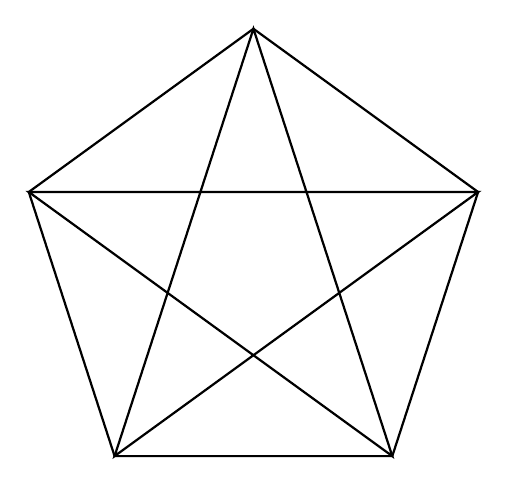
\begin{tikzpicture}
    % Define the five vertices of the pentagon
    \foreach \i in {1,2,3,4,5} {
        \coordinate (P\i) at (90+72*\i:3);
    }

    % Draw the pentagon
    \draw[thick] (P1) -- (P2) -- (P3) -- (P4) -- (P5) -- cycle;

    % Draw the star by connecting alternate vertices
    \draw[thick] (P1) -- (P3) -- (P5) -- (P2) -- (P4) -- cycle;

\end{tikzpicture}

I found the invariant, the sum of the vertices, actually just do an indicator function whether the vertex is 1 or 0. Everytime you dojjj 
a move, it always interacts with two of the vertices on the outside, and preserves the parity, the case of having all -1, corresponds to 
having 0, but that has different parity from 5, so it is impossible.

What What about the case of a hexagon?


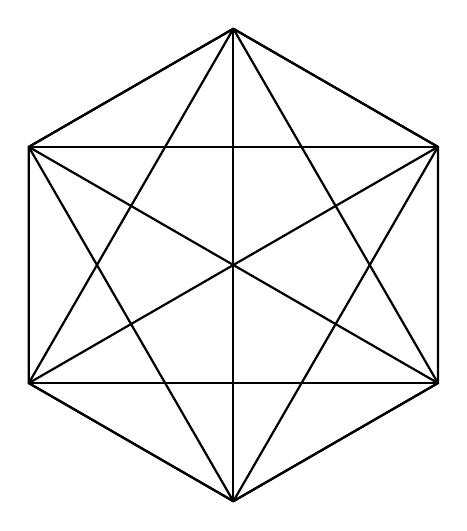
\begin{tikzpicture}
    % Define the six vertices of the hexagon
    \foreach \i in {1,2,3,4,5,6} {
        \coordinate (H\i) at (90+60*\i:3);
    }

    % Draw the hexagon
    \draw[thick] (H1) -- (H2) -- (H3) -- (H4) -- (H5) -- (H6) -- cycle;

    % Draw all diagonals (connecting every pair of vertices)
    \foreach \i in {1,2,3,4,5,6} {
        \foreach \j in {1,2,3,4,5,6} {
            \ifnum\i<\j
                \draw[thick] (H\i) -- (H\j);
            \fi
        }
    }

\end{tikzpicture}

I must say it looks, beautiful. It feels like there is so much freedom. But there are 19 points in total.
Now I am feeling extra fishy. Let me think on it.

Ok I couldn't find a solution using the same trick as before? What about a different?
The function I make must have some nonzero coeffiecient for the center. There is also the problem
that there moves that intersect 2, and 5 nodes. And I would have to treat the center the same as 
the ones on the middle of the side of the center hexagons.

Maybe it is possible....

After reading the book, it said the product of the number on the nine circles doesn't change?

What did I learn? Consider product when doing invariants, especially mod 2, and any collection of 
odd objects with even intersection works.

\begin{figure}[h]
    \centering
    
\includegraphics[width=0.5\textwidth]{pic1.png}
    \label{fig:example}
\end{figure}


\subsection{Problem 48}

In Fig. 1.7, two squares are neighbors if they have a common boundary. Consider
the following operation \( T \): Choose any two neighboring numbers and add the same
integer to them. Can you transform Fig. 1.7 into Fig. 1.8 by iteration of \( T \)?

\begin{center}
    \textbf{Fig. 1.7}
    
    \[
    \begin{bmatrix}
        1 & 2 & 3 \\
        4 & 5 & 6 \\
        7 & 8 & 9
    \end{bmatrix}
    \]
\end{center}

\begin{center}
    \textbf{Fig. 1.8}
    
    \[
    \begin{bmatrix}
        7 & 8 & 9 \\
        6 & 2 & 4 \\
        3 & 5 & 1
    \end{bmatrix}
    \]
\end{center}

\textbf{Solution}

This is the checkerboard problem, first color it like a checker board and see if the difference in the total sum of all 
white and black cells of the first box mathes that of the second. Then if they do match you turn the first one by first 
fixing the top left $2\times 2$ box and you can do this first fixing the top left and then using the same technique to go down.
Then in the last row fix every number and the last two must be the same in the box since the difference has to be the same so you can 
either increase the two numbers to match or it decrease them. 

I don't want to check specifically, oh well I will then.

The first one is(top left is assumed to be black): 1+3+5+7+9, the white is 2+4+6+8=15-20=5
The second one is: 7+9+2+3+1, white is 8+4+6+5. So the difference is 22-23=-1

Unfortunately $-1 \neq 5$, basically the invaraint is the difference in the sum of white squares and black squares.

\subsection{Problem 49}

There are several signs + and - on a blackboard. You may erase two signs and
write, instead, + if they are equal and - if they are unequal. Then, the last sign on
the board does not depend on the order of erasure.

\textbf{Solution}

Is the product just conserved? It literally is!

Ok could I do it with XOR? Isn't that also just checking the parity as well. I guess there is nothign then.

\subsection{Problem 50}

There are several letters $e,\;a$ and b on a blackboard. We may replace two e's by one
e, two a's by one b, two b's by one a, an a and a b by one e, an a and an e by one
a, a b, and an e by one b. Prove that the last letter does not depend on the order of
erasure.

\textbf{Solution}

I have to make the recurrence funciton. I also need to write down the funcitions because this 
is just too confusing.

$a$ is the number of a's, and henceforth for all the other letters.

\begin{align*}
    (a,b,e) \rightarrow (a,b,e-1)\\
    (a,b,e) \rightarrow (a-2,b+1,e)\\
    (a,b,c) \rightarrow (a+1,b-2,e)\\
    (a,b,c) \rightarrow (a-1,b-1,e+1)\\
\end{align*}

The question has a lot of detours since the three of the operations are the same.

The difference between $a$ and $b$, mod 3, doesn't change so the if the difference between them mod 3,
then the final choce has be e. Or basically $S=a-b+0*e mod 3$ is invariant. But I need to find the 
values of the final chip when it isn't the case that the dfference isn't mod 3 is 0. What if I do $S=2a+2b mod 3$,
when $a$ decreases by 2, and b increases by 1, does it still become invariant? a's change becomes a decrease of 1 mod 3, and
b's increase becomes 2 in mod 3. So S should stay invariant. Actually this doesn't matter 
since I can't use this to tell apart a and b. Since decreasig from $a$ and decreasig from $b$ are symmetric,
their interations must be similar,and their coefficeints equal. Actually I think $S=a-b$ suffices.
If $S=0$, then it is e, if $1$ then it is a, if $2$, then it is b. This is also a criteria for there to only exist one chip lest in the end.

How do I make sure this is true. Since the invariant is constant, if there is a one chip at the end, if it is e, then S must have been 0. 
If S=1, then there is one a chip and if it is 2, then that means there is one b chip since $2 \equiv -1 mod 3$. 

Actually after reading the book it had a very cool proof. 


\[
e \circ e = e, \quad e \circ a = a, \quad e \circ b = b, \quad a \circ a = b, \quad b \circ b = a, \quad a \circ b = e.
\]

The \(\circ\) operation is commutative since we did not mention the order. It is easy to check that it is also associative, i.e.,

\[
(p \circ q) \circ r = p \circ (q \circ r)
\]

for all letters occurring. Thus, the product of all letters is independent of the order in which they are multiplied.

\subsection{Problem 51}
A dragon has 100 heads. A knight can cut off 15, 17, 20, or 5 heads, respectively,
with one blow of his sword. In each of these cases, 24, 2, 14, or 17 new heads grow
on its shoulders. If all heads are blown off, the dragon dies. Can the dragon ever die?

\textbf{Soltion}

Let h represent the number of heads.

So the operations I can do are

\begin{align*}
  h \wedge h\geq 15 \rightarrow h+9 \\
  h \wedge h\geq 17 \rightarrow h-15 \\
  h \wedge h \geq 20\rightarrow h-6 \\
  h \wedge h \geq 17 \rightarrow h+15 
\end{align*}

I think is also dies if the number of heads is less or equal to 20. Since I 
can hit it and it will die.

If the requirement is only all of the heads are blown off until it dies, then it can be killed by just used blowing 20 heads each time.

If exactly 0 heads must exist at a time then it is impossible because it has each move preserves the mod 3 parity, and the number of 
heads I must chop off need to have 0, and 2 and mod 3 but 100 has 1 mod 3.

\subsection{Problem 52}


Is it possible to arrange the integers \(1, 1, 2, 2, \dots, 1998, 1998\) such that there are exactly \(i - 1\) other numbers between any two \(i\)'s?

\textbf{Solution}

This is like the codeforce blog. I will think about it later because is 3:11 PM, and I need to sleep.

So let's say the indices of the numbers are $i_{11},i_{12},i_{21},i_{22},\cdots$. The difference added up should give the below expression.

\begin{align*}
  (i_{21}-i_{11}) + (i_{22}-i_{21}) + \cdots = (0) + (1) + (2) + \cdots + 1997\\
\end{align*}

If you take this mod 2, then $a-b \equiv a+b mod 2$. So 

\begin{align*}
  i_{11} + \cdots = \frac{1998*1997}{2} = 999*1997
\end{align*}

Since the sum of all the doubles of the numbers on the left is odd, the sum is even and the one on the right is wrong therefore the 
sequence can't exist. 

Would this proof for cases where I was asked an odd number? Actually it depends on the mod 4. When the final value mod 4 is 3, then once I add one and divide
I get an odd number, therefore the proof works in that case. Wait I mean when the final number(1998) mod 4 is 2, I can do this proof. So for all numbers with 
mod 4, you can't do this process, what about 0,1,3? In the case of 0, it will be divisible and the proof will not work. In the case of 1? It will also fail, in the case of 3? It will work. SO for all numbers who have mod 4, 2,3 and this will proof will work, and it is impossible.

\subsection{Problem 53}


The following operations are permitted with the quadratic polynomial \( ax^2 + bx + c \):
\begin{itemize}
    \item[(a)] Switch \( a \) and \( c \).
    \item[(b)] Replace \( x \) by \( x + t \), where \( t \) is any real number.
\end{itemize}
By repeating these operations, can you transform \( x^2 - x - 2 \) into \( x^2 - x - 1 \)?

\textbf{Solution}

The discriminant is conserved, I did a question like this before. The discriminant of the two quadratics aren't the same.
The book actually has an elegant point about what the discriminant is. It is the difference between, and another insight I didn't 
think about before is that the min or max of the quadratic function is between the roots, so $\frac{-b}{2a}=\frac{x_1+x_2}{2} \rightarrow \frac{-b}{a}=(x_1+x_2)$.


This is an invariance problem. As a prime candidate, we think of the discriminant \( D \). 
The first operation obviously does not change \( D \). The second operation does not change 
the difference of the roots of the polynomial.

Now, 
\[
D = b^2 - 4ac = a^2 \left( \left( \frac{b}{a} \right)^2 - 4 \frac{c}{a} \right),
\]
but 
\[
-\frac{b}{a} = x_1 + x_2, \quad \text{and} \quad \frac{c}{a} = x_1 x_2.
\]
Hence, 
\[
D = a^2 (x_1 - x_2)^2,
\]
i.e., the second operation does not change \( D \). 

Since the two trinomials have discriminants \( 9 \) and \( 5 \), the goal cannot be reached.

\subsection{Problem 54}

Initially, we have three piles with \( a \), \( b \), and \( c \) chips, respectively. In one step, you may 
transfer one chip from any pile with \( x \) chips onto any other pile with \( y \) chips. 

Let 
\[
d = y - x + 1.
\]
If \( d > 0 \), the bank pays you \( d \) dollars. If \( d < 0 \), you pay the bank \( |d| \) dollars. 

Repeating this step several times, you observe that the original distribution of chips has been restored. 

What is the maximum amount you can have gained at this stage?

\textbf{Solution}

So d is the old value of $x$ - new value of $y$. Does it have any deeper meaning?
Ok, what should I do then? I want find the maximum amount of money I got? I feel that this should be 0, 
but I am not sure let me think about, I will sleep now, since it is 3:19.

I couldn't figure the how it actually worked but, the invarint is $a^2 + b^2+ c^2- 2*g$. How should I be 
able to recognize? the combinaiton should have looked, and I should look for invariants to make it zero.

\subsection{Problem 55}


Let \( d(n) \) be the digital sum of \( n \in \mathbb{N} \). Solve the equation:

\[
n + d(n) + d(d(n)) = 1997.
\]


\textbf{Solution}

Since the digit summed is conserved under module 9, and the we have to be able to find the inverse of 
$1997 mod 9$, which is the inverse of $8$ in mod 9. Actually we want something times 3, to give 8 in module 9.
So it is impossible, the book said the transformation is invariant under modul 3.
Actualy I get it now, since the sum of the digits is used to check divisibilty for 3, which we can use it to 
know that d is invariant under module 3. So the equation becomes $0\equiv 2 mod 3$, whcih is impoosible. 
That was simpler than my proof.

\subsection{Porblem 56}


Start with four congruent right triangles. In one step, you may take any triangle and cut it in two with the altitude from the right angle. Prove that you can never get rid of congruent triangles.


\textbf{Solution}

I actually couldn't solve this question, it was quite tricky to get the formulas correct, the books insight was 
that you can desscribe the first traingle as $1,p,q$ where $1 \geq q, p$ and then all the next traingles will be 
with coefficients of $p^m q^n$. Then you can use the same lattice point with powers of 2 technique in question 39, 
to show that you can't have four all the points be distinct on the lattice points without filling up the entire plane with would require infinite moves.

\subsection{Problem 57}

Starting with a point \( S(a, b) \) of the plane with \( 0 < a < b \), we generate a sequence \( (x_n, y_n) \) of points according to the rule:

\[
x_0 = a, \quad y_0 = b
\]

\[
x_{n+1} = \sqrt{x_n y_{n+1}}, \quad y_{n+1} = \sqrt{x_n y_n}.
\]
Prove that there is a limiting point with $x=y$. Find this limit.


\textbf{Solution}

What could the invariant be? Could it be in the example with the product being fixed and the end result 
having something to do with cosine?

The value $x_{n+1}\sqrt{y_{n+1}}=x_{n}\sqrt{y_{n}}$.
The values of $y$ are decreasign and the values of $x$ are increasing, and  the values stay constant 
after reaching $x=y=(a^2 b)^{1/3}$.

Actually I didn't rigoursly prove that x is increasing and y is decreasing. But the book had an interesting 
point on the relationship between the geometric mean, and the arthimetic mean. The arthimetic mean is always bigger.

\subsection{Problem 58}


Consider any binary word \( W = a_1 a_2 \cdots a_n \). It can be transformed by inserting, deleting, or appending any word \( XXX \), where \( X \) is any binary word. Our goal is to transform \( W \) from \( 01 \) to \( 10 \) by a sequence of such transformations. 

Can the goal be attained? (LMO 1988, oral round)

\textbf{Solution}

Can I do this? The ones I remove will have to be a 3 repetition and the ones I add will also have to be 3 repetitions.
What is conserved when I do this operation?



\end{document}
